\chapter{Software Defined Radio}

Software Define Radio, SDR is a radio communication system where most of the 
hardware components have been replaced by software \cite{wikiSDR}. This isn't
a new concept but recent advances in electronics technologies have made many
things possible that were just theoretically possible before. In traditional
radio systems, all the components are hardwired into the device. These 
components cannot be modified or tweaked easily. Most of them needs to be 
replaced instead. They are also much more expensive to reconfigure. But in an
SDR, to change the functionality of the radio system all you need to do is
rewrite its software. Thus it can be reconfigured easily and economically.
The protocols used by the software based radio system can also be changed
easily. Usually, in an SDR most of the hard work is handed over to a general
purpose microprocessor instead of a special purpose hardware.

The traditional hardware radio system consists of elements such as mixers, 
filters, amplifiers, converters, modulators, etc. resulting in higher 
production costs and minimal flexibility. Whereas in SDR technologies like 
Field Programmable Gate Array (FPGA), Digital Signal Processor (DSP) and 
General-Purpose Processor (GPP) are used to build the software radio elements.


\begin{figure}
  \centering
  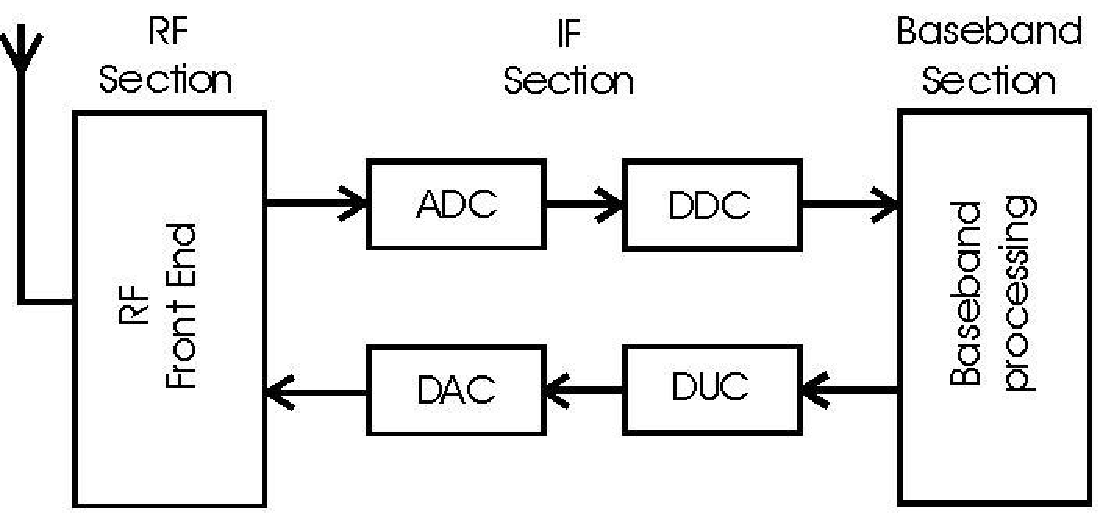
\includegraphics[width=0.7\textwidth]{../images/sdrBlock}
  \caption{Block diagram of SDR.}
  \label{sdrBlock}
\end{figure}

The SDR contains a number of basic functional blocks.
The SDR in general can be divided into three basic sections, namely the front
end, the IF section and the base-band section. The front end section consits 
of analogue RF circuitry that is responsible for the reception and 
transmission of signals at the operating frequency. The IF section performs
the digital to analog conversion and vice versa. It also does various signal 
processing tasks like filtering, modulation and demodulation, digital up 
conversion (DUC), digital down conversion (DDC) etc. The last stage of the 
radio is the baseband processor. It is at this point that the digital data 
gets processed \cite{miller08}\cite{kranthi13}.
We have used GNURadio and USRP N210 to configure the SDR used in implementing
our Cognitive Radio testbed. 

\begin{figure}
  \centering
  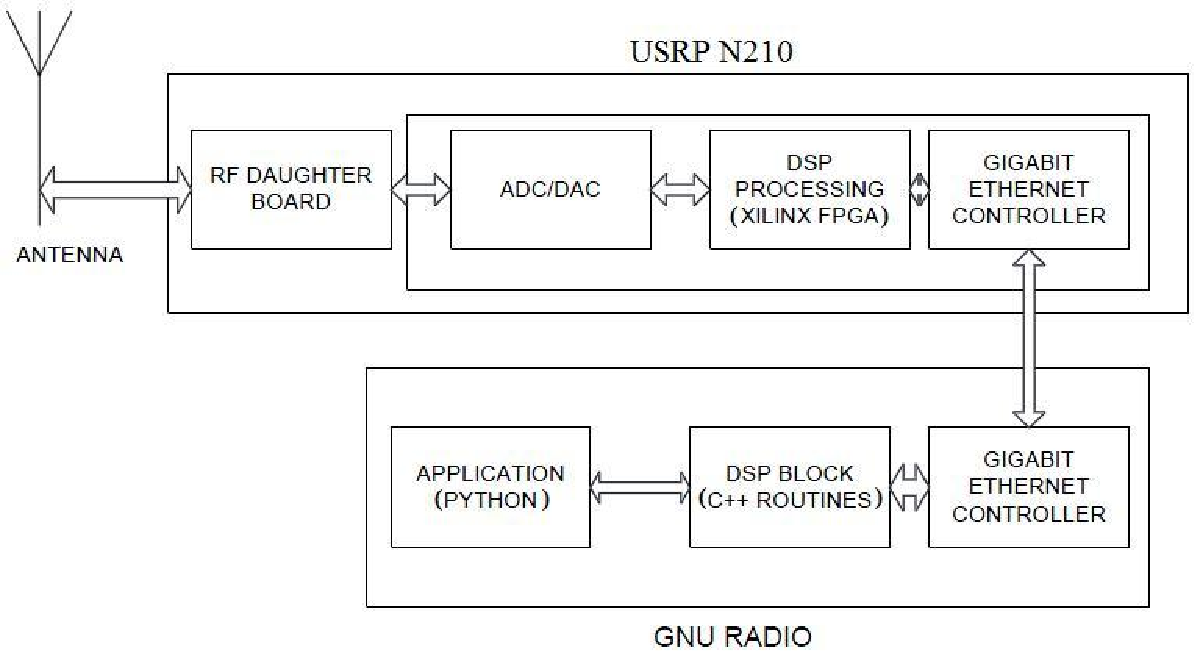
\includegraphics[width=0.7\textwidth]{../images/usrpGNURadioBlock}
  \caption[USRP operation with GNURadio]{Block diagram for the operation of USRP
  with GNURadio.}
  \label{usrpGNURadioBlock}
\end{figure}

A block diagram of a USRP-based SDR transceiver executing a GNURadio based 
application is shown in Figure \ref{usrpGNURadioBlock}. The USRP kit is the 
hardware interface and GNURadio is used for the baseband signal processing
tasks.


\section{USRP}

The USRP (Universal Software Radio Peripheral) is intended to provide a 
low-cost, high quality hardware platform for software radio. It is designed
and marketed by Ettus Research, LLC. It is commonly used by research labs,
universities, and hobbyists. The USRP platform is designed for RF applications
from DC to 6 GHz. USRPs connect to a host computer through a high-speed USB or
Gigabit Ethernet link, which the host-based software uses to control the USRP
hardware and transmit/receive data.

The USRP Hardware Driver (UHD) is the official driver for all Ettus Research
products. The UHD supports Linux, Mac OS X and Windows.

\begin{figure}
\centering
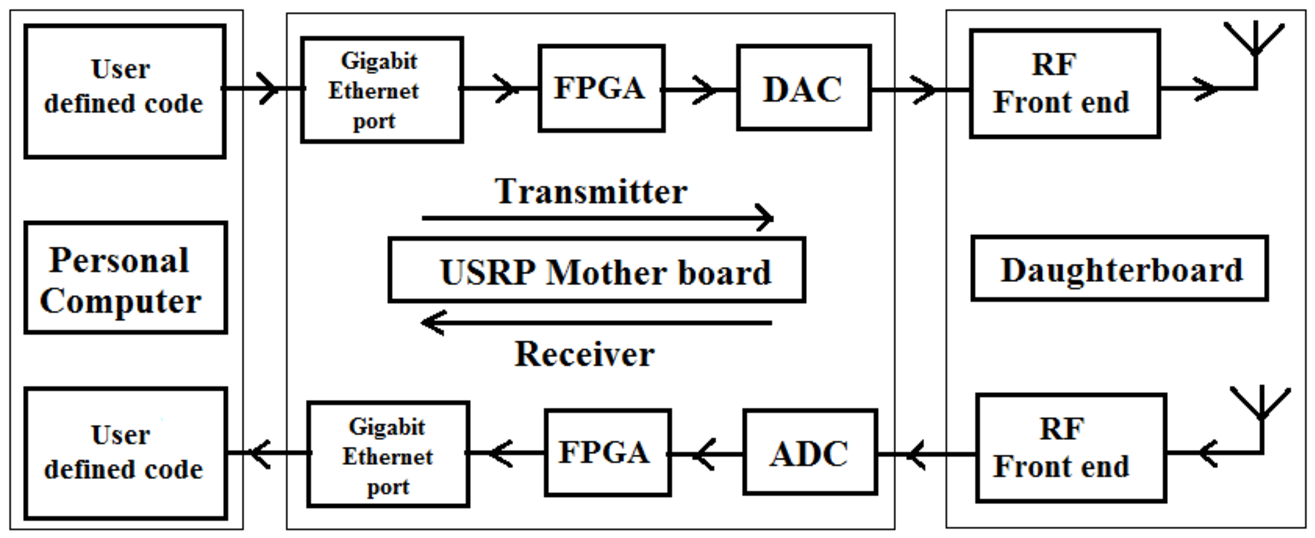
\includegraphics[width=0.9\textwidth]{../images/usrpBlock}
\caption[Block diagram of USRP]{Block diagram of USRP 
\protect\cite{kranthi13}.}
\label{usrpBlock}
\end{figure}

In this project we are using a particular model of USRP product known as the
USRP N210.

\subsection{USRP N210}

The USRP N200 and N210 are the highest performing class of hardware of the 
USRP family of products, which enables engineers to rapidly design and 
implement powerful, flexible software radio systems. The N200 and N210 
hardware is ideally suited for applications requiring high RF performance and
great bandwidth. Such applications include physical layer prototyping, dynamic
spectrum access and cognitive radio, spectrum monitoring, record and playback,
and even networked sensor deployment. The Networked Series products offers 
MIMO capability with high bandwidth and dynamic range. The Gigabit Ethernet
interface serves as the connection between the N200/N210 and the host 
computer. This enables the user to realize 50 MS/s of real-time bandwidth in 
the receive and transmit directions, simultaneously (full duplex).


\section{GNU Radio}

GNU Radio is a free \& open-source software development toolkit that provides 
signal processing blocks to implement software radios. It can be used with 
readily-available low-cost external RF hardware to create software-defined 
radios, or without hardware in a simulation-like environment. It is widely 
used in hobbyist, academic and commercial environments to support both 
wireless communications research and real-world radio systems.

\subsection{What does GNU Radio do?}
It does all the signal processing. You can use it to write applications to 
receive data out of digital streams or to push data into digital streams, 
which is then transmitted using hardware.

GNU Radio has software equivalents of real world radio system components like 
filters, demodulators, equalizers, etc. These are usually referred to as
blocks. You can create a complex system by connecting various blocks. If you
cannot find some specific blocks, you can even create your own blocks and add
them.

Most of GNU Radio has been implemented using the Python programming language,
and the performance-critical parts have been implemented using C++. Typically,
a GNU Radio user writes his applications in Python, unless he has some
performance-critical needs. Thus, GNU Radio gives its users an easy-to-use,
rapid application development environment.

\subsection{GNU Radio with USRP}

\begin{figure}
\centering
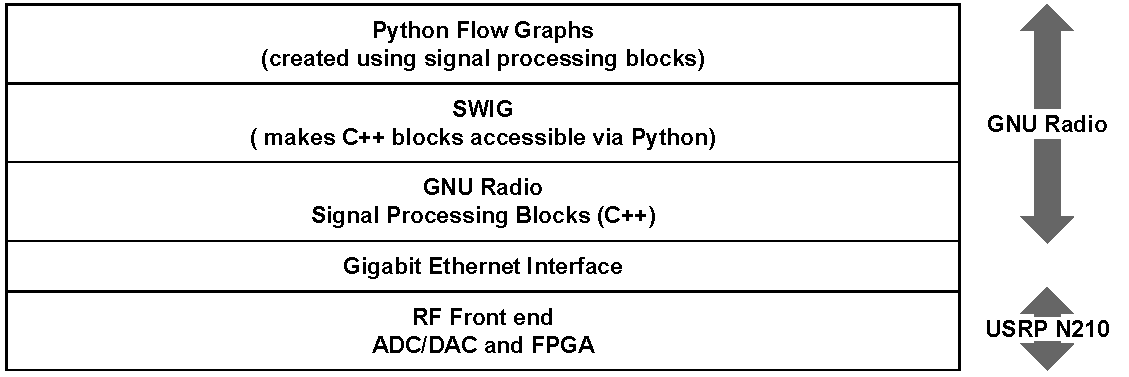
\includegraphics[width=0.9\textwidth]{../images/gnuradio_architecture}
\caption{Architecture of GNU Radio}
\label{gnuradio_architecture}
\end{figure}

The USRP and the host computer make up the hardware part of the SDR system. 
The host computer must run a compatible software package such as GNU Radio or
Simulink to complete the SDR system. In this project we are using GNU Radio
as the software platform.

GNU Radio communicates with the USRP through the USRP Hardware Driver (UHD)
software. The UHD provides a host driver and an Application Programming
Interface (API) for the USRP. GNU Radio uses the UHD to set user-specified
parameters like RF center frequency, antenna selection, gain, sampling rate,
interpolation, decimation, etc.

